\chapter*{Introduction}
\markboth{Introduction}{}
\label{cap:introduction}
\addcontentsline{toc}{chapter}{Introduction}

\section{Motivation}
\label{sec:mt}

The main motivation for which we have decided to undertake this project is that, according to ~\cite{wearesocial2024}, a large volume of data is moved on social networks (measurable on the scale of exabytes), they have a massive number of users, exceeding 5 billion active users, and an average usage time of 2 hours and 23 minutes per day, but we spend an average of 6 hours and 40 minutes online daily. Furthermore, the most widely used social network in 2024 was TikTok, which is based on short-duration videos, allowing videos of up to 60 seconds in its origins and currently up to 60 minutes. This makes the transmission of secret information through videos with audio on the public network go unnoticed due to its abusive but common use today. 


\begin{figure}[h]
	\centering
	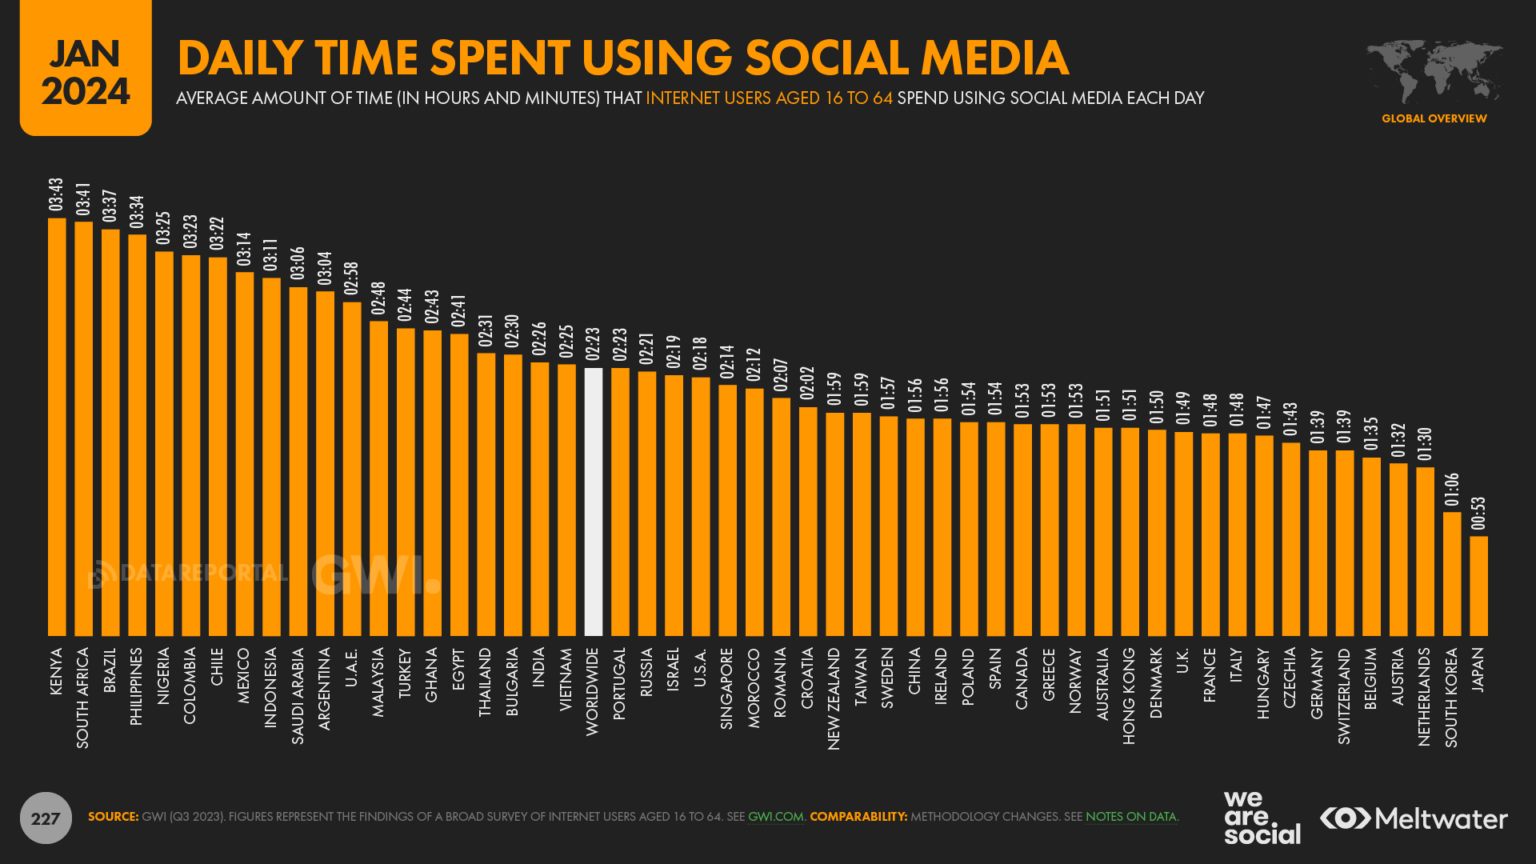
\includegraphics[width = 0.8\textwidth]{Imagenes/pitea/grafica_tiempo_redes_sociales.png}
	\caption[Social media usage time by country]{Graph of social media usage time by country. ~\cite{wearesocial2024}.}
	\label{fig:proceso}
\end{figure}

To avoid confidentiality risks in the data, the use of steganography becomes fundamental, which will be introduced in more detail in this document, but for now, we will define it as techniques for hiding information, to ensure that if someone obtains a video legally or illegally, they are unable to detect that it contains valuable information, as this is hidden and appears to be just another video in the sea of bytes.

 

\section{Objectives}
The objective of this project is to develop a tool capable of using methods for transforming text into images and images into audio in order to transmit information secretly and take advantage of the intense use of social networks that exists today.  

To achieve this, we will focus on: 

\begin{itemize}
    \item Creation of a CLI (Command-line interface).
    \item Implementation of algorithms for hiding and revealing both text in images and images in audio.
    \item Processing of acoustic waves in computing.
    \item Use of secret key cryptography.
\end{itemize}

\section{Work plan}

In this section, the detailed work plan is described with which it is expected to achieve the project's objectives.

\subsection{Stage 1: Preliminary Research }

\textbf{Objective:} Conduct preliminary research before the development of the tool in order to become familiar with the necessary knowledge and techniques.\\

\textbf{Tasks:}
\begin{itemize}
    \item Search for information on steganography and cryptography. 
    \item Search for information on multimedia file encoding.  
    \item Analyze existing tools.
\end{itemize}



\subsection{Stage 2: Development of a Basic Functional Prototype}
\textbf{Objective:} Create a functional prototype of the tool that performs hiding and uncovering using LSB (Least Significant Bit).\\

\textbf{Tasks:}
\begin{itemize}
    \item Develop a sequential program that carries out the complete process of hiding and uncovering.
    \item Implement basic functionalities, such as encrypting text using AES and hiding the text and image using the LSB hiding method. 
    \item Conduct tests to verify that the basic system functions correctly and that the information is not modified in the process.
\end{itemize}



\subsection{Stage 3: Modularization and Enhancement of Functionalities}
\textbf{Objective:} Modularize the program and add additional functionalities, such as generating audio from images to transmit them via SSTV.\\

\textbf{Tasks:}
\begin{itemize}
    \item Divide the code into modules by making appropriate use of OOP (Object-Oriented Programming) to separate the responsibilities of encryption, steganography in images, steganography in audio, and handling inputs and outputs. 
    \item Implement additional functionalities, such as the ability to choose between different concealment techniques. 
    \item Conduct integration tests to ensure that the modules work well together.  

\end{itemize}

\subsection{Stage 4: Creation of the CLI  }
\textbf{Objective:} Create the command-line interface to facilitate interaction with the program.\\

\textbf{Tasks:}
\begin{itemize}
    \item Implement the command-line interface.  
    \item Integrate the interface with the previously developed modules. 
    \item Ensure that users can only choose possible execution flows.  
\end{itemize}

\subsection{Stage 5: Tool Testing }
\textbf{Objective:} Conduct tests on the tool to ensure reliability and discover the limitations of the system.\\ 

\textbf{Tasks:}
\begin{itemize}
    \item Carry out tests to check the reliability of the tool by using it in real use cases.
    \item Conduct tests to study the limitations of the tool. 
\end{itemize}


\subsection{Stage 6: Documentation}
\textbf{Objective:} Document the architecture of the tool as well as the conclusions we have reached.\\

\textbf{Tasks:}
\begin{itemize}
    \item Create detailed documentation on the code, functionalities, usage of the tool, its installation, the technologies used, and also those discarded. 
    \item Prepare a presentation to showcase the project and its final results.  
\end{itemize}









